\chapter{Datos y metodología}
\label{chapter:datos_metodologia}
\section{Datos: La Encuesta Financiera de las Familias}

Los datos que se van a utilizar en este proyecto provienen de la Encuesta Financiera de las Familias (EFF). La EFF es una encuesta oficial a hogares elaborada por el Banco de España y está incluida en el Plan Estadístico Nacional. Su primera edicion se realizó en el año 2002, y se ha producido de manera trienal hasta el año 2020. Desde entonces, se produce de manera bienal.

El objetivo de la EFF es recabar información sobre las condiciones financieras de los hogares residentes en España. Es la única fuente estadística que permite relacionar información sobre activos, deudas, ingresos y gastos de los hogares españoles. Esto permite analizar las decisiones de inversión y financiación de las familias y conocer su situación patrimonial, y gracias a ello tener un mayor conocimiento de la economía española y ser un apoyo importante para el diseño de politicas públicas. Por nombrar algunos ejemplos de estudios realizados con la EFF, se ha utilizado para cuantificar el ahorro adicional generado para los partícipes en planes de pensiones de empresa (\cite{gomez2022pensiones}), para caracterizar cómo afectó la pandemia del Covid-19 a la situación patrimonial de los trabajadores más afectados por dicha crisis (\cite{alvargonzalez2020pandemia} o para analizar las diferencias en aceptación y uso de tarjetas de crédito y banca online entre diferentes grupos de hogares desde el año 2002 (\cite{crespo2023bancaonline}).

El diseño de la muestra de la EFF tiene dos características importantes: un sobremuestreo de hogares ricos y un componente longitudinal o panel. El sobremuestreo de ricos\footnote{La muestra de la EFF es seleccionada por el Instituto Nacional de Estadística, en colaboración con la Agencia Tributaria, a partir de las declaraciones individuales más recientes en el Impuesto sobre el Patrimonio. Los detalles sobre el muestreo de la EFF pueden consultarse en los documentos metodológicos disponibles en su \href{https://app.bde.es/efs_www/home?lang=ES}{sitio web}.} garantiza poder analizar con suficiente precisión el comportamiento de los hogares de la parte alta de la distribución de riqueza. Este detalle es importante porque la distribución de la riqueza entre los hogares es asimétrica, por lo que sólo unos pocos hogares, especialmente los más ricos, son los que invierten en ciertos activos. Por otro lado, el compomente panel indica que se vuelve a entrevistar a hogares que participaron en ediciones anteriores. Esto permite monitorearles durante períodos de hasta diez años, y observar los cambios en las variables de interés de la encuesta. El número máximo de ediciones en las que un hogar puede participar en la EFF es de cuatro olas consecutivas. Si cesa su participación antes de completar sus cuatro ediciones, se descarta de la muestra y no vuelve a ser contactado en olas posteriores. Finalmente, para poder combinar ambas características y mantener la representatividad de la muestra para cada edición, en cada ola nueva se incluye una muestra de refresco con hogares nuevos.

En este proyecto vamos a utilizar datos que provienen tanto de las respuestas de los hogares al cuestionario de la EFF, como del paradata recopilado durante la elaboración de la encuesta. Para esto, es importante comprender bien cómo es el proceso de producción de la EFF y los datos que éste genera más allá de las respuestas de los hogares. Éste proceso puede verse de manera visual y resumida en la figura 4.1. La producción de la EFF se divide en dos grandes fases: Campo y Post-Campo. Durante la fase de Campo se contacta con los hogares, se realiza la entrevista personal, se procesan los datos y se realiza parte de la revisión de los mismos. En el Post-campo se termina el proceso de revisión, se revisa el grado de no-respuesta que hay en los datos, y se procede a la imputación de todas esas variables. Tras la imputación, se obtienen los datos finales. A continuación vamos a comentar con más detalle y en orden cronológico algunos aspectos de estas fases.

\begin{figure}[h]
	\centering
	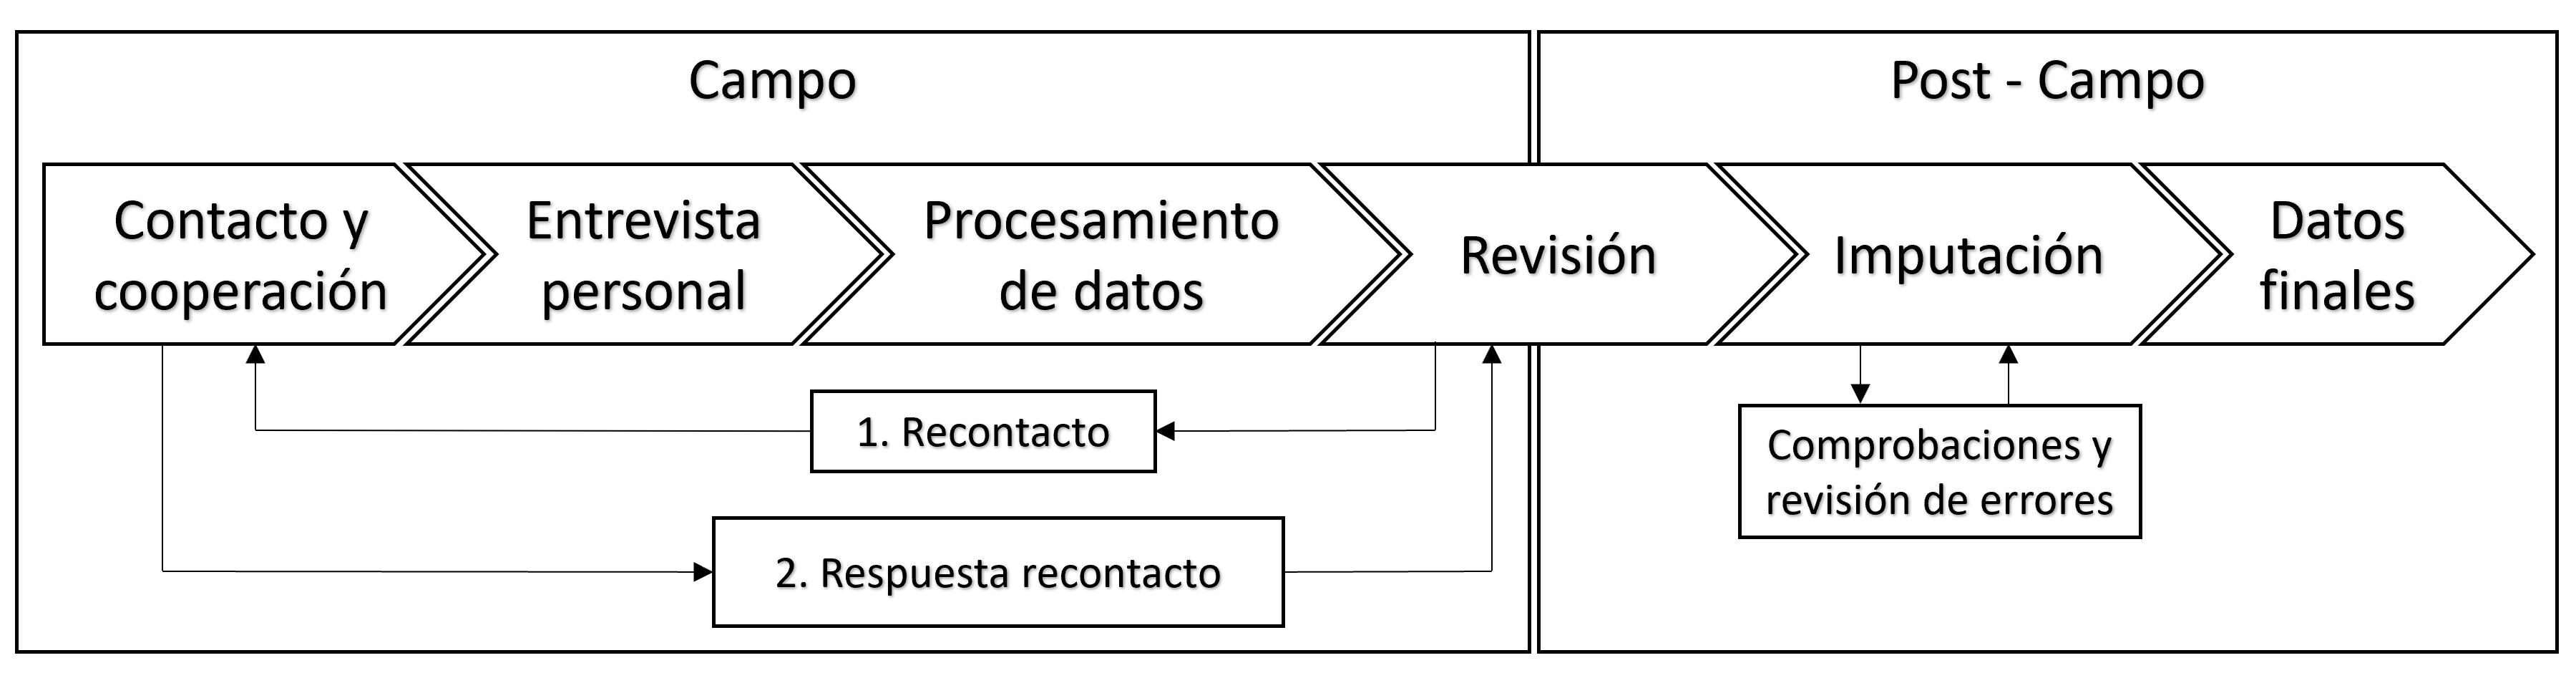
\includegraphics[width=1\textwidth]{figs/fases_creacion_datos_eff.png}
	\caption{Fases de la creación de datos de la EFF}
	\label{fig:eff_phases}
\end{figure}

Para establecer el contacto, los entrevistadores realizan visitas personales a los hogares en sus domicilios. Esto puede requerir varios intentos, ya que es necesario que algún miembro del hogar esté físicamente en su hogar cuando tenga lugar la visita presencial. A continuación, se realiza una entrevista personal a la persona con más conocimiento de las finanzas del hogar, que se denomina Persona de Referencia o PR. La PR puede ser miembro del hogar, o un representante del mismo, demoninado proxy, siempre y cuando sea la persona con mayor conocimiento de las finanzas del hogar. También pueden participar en la entrevista otros miembros del hogar. Al principio de la entrevista, se pide a la PR su conformidad para grabar la entrevista en audio por motivos de calidad de los datos. Si se niega, la entrevista continúa, pero su revisión no dispondrá de audios. Los entrevistadores recogen las respuestas en un ordenador o una tablet (CAPI), y también anotan con comentarios de texto todos los detalles que consideren importantes para la revisión. La PR puede decidir no contestar a ciertas preguntas. Su valor se asignará como missing, y se imputará más adelante.

Adicionalmente, y sin la presencia de los hogares, los entrevistadores rellenan dos cuestionarios adicionales. Uno para recoger información sobre las características del vecindario y el tipo de edificio en el que vive el hogar, y otro con información sobre el desarrollo de la entrevista, como por ejemplo el nivel de interés mostrado por la PR o el nivel de entendimiento percibido de las preguntas.

Es necesario mencionar que algunos elementos de este procedimiento se modificaron durante la EFF2020, ya que el campo empezó en noviembre de 2020 y se vió afectado por la pandemia del Covid-19. Durante esa ola, los entrevistadores siguieron visitando personalmente a los hogares para conseguir su colaboración\footnote{Durante el principio del campo, algunos hogares panel fueron contactados sólo por teléfono, pero a las pocas semanas se decidió establecer la visita personal como el procedimiento estándar.}, pero siempre respetando las medidas de distancia social. Las entrevistas se realizaron de manera telefónica asistida por una tablet (CATI). El resto del procedimiento se mantuvo.

Tras terminar la entrevista, todos los datos son procesados y enviados al equipo de revisión, que revisa individualmente todas las entrevistas y corrige los errores que puedan detectarse. Si se considera que hay información que se ha recogido erróneamente o se ha omitido, se recontacta con el hogar puede para corregir o recuperar esa información. Este recontacto se hace por teléfono. Tras este proceso de revisión, se analiza la proporción de preguntas sin responder de cada entrevista, y se eliminan las que no superen ciertos umbrales de calidad. Finalmente, todas las variables que contienen no-respuesta se imputan mediante técnicas de imputación múltiple\footnote{Los métodos de imputación múltiple utilizados en la EFF pueden consultarse en \cite{barcelo2006imputation}}.

Para la elaboración de este proyecto se utiliza información recopilada durante las olas de la EFF2017, EFF2020 y EFF2022. La razón para elegir sólo estas ediciones es que son las únicas que cuentan con información detallada de paradatos y de las características de los entrevistadores. Para ediciones anteriores, esta información o no está disponible o contiene grandes errores de medida. A pesar de esto, es posible identificar el número de ediciones en las que ha participado cada hogar, por lo que es posible utilizar información que se remonta hasta la edición de la EFF2011.

A continuación se enumeran los ficheros de datos que se han utilizado durante este proyecto:

\begin{itemize}
    \item Fichero de trabajo con respuestas de los hogares: Registro de hogares que contiene las respuestas al cuestionario justo antes de la imputación. Incluye las variables que contienen no-respuesta.
    \item Fichero de datos imputados: Registro de hogares que contiene las respuestas al cuestionario después de la imputación. Por simplicidad, sólo utilizaremos uno de los conjuntos de datos de la imputación multiple.
    \item Fichero de contactos: Registo de hogares que contiene la información sobre el proceso de contacto con el hogar y sus resultados. Incluye el número de intentos de contacto, la fecha en que se produjo y el resultado de cada uno de ellos (aplazamientos, rechazos...).
    \item Fichero de recontactos: Registro de hogares que contiene información sobre el proceso de revisión y los recontactos.
    \item Censo de entrevistadores: Registro de entrevistadores que contiene la información disponible sobre los entrevistadores que han participado desde la EFF2014 a la EFF2022.
    \item Fichero de paradata: Registro de las pantallas del software CAPI o CATI. Para cada hogar, contiene información detallada de la interacción del entrevistador con el ordenador durante la entrevista. En concreto, contiene el flujo de pantallas que se visualizaron en el ordenador en cada entrevista y el tiempo que se estuvo en cada una.
\end{itemize}

\section{Metodología}

Tomando como referencia las estrategias de investigación propuestas en \cite{oates2022researching}, en este proyecto se sigue la estrategia de 'Caso de estudio', ya que se busca tener un conocimiento profundo sobre la participación de los hogares panel en el caso específico de la EFF, y buscar maneras de tratarlo. En concreto, vamos a intentar adaptar la implementación hecha por \cite{beste2023case} al caso de la EFF.

El objetivo es predecir si un hogar que ha participado en la ola $t$ no volverá a participar en la siguiente ola $t+1$. Para ello, se define una variable objetivo dicotómica Attrition que toma valor 0 si el hogar vuelve a participar, y valor 1 si no vuelve a participar:

\begin{equation}
Attrition =
  \begin{cases}
    0       & \quad \text{el hogar participa en la ola $t+1$} \\
    1  & \quad \text{el hogar no participa en la ola $t+1$}
  \end{cases}
\end{equation}

La metodología de este proyecto se fundamenta en cuatro pilares: La recopilación de los datos de los hogares y los entrevistadores que participaron en las ediciones de 2017, 2020 y 2022 de la EFF, la selección de variables para los modelos de predicción a través de un análisis cualitativo y cuantitativo, el entrenamiento de varios modelos basados en métodos de machine learning con datos de la EFF2017 y la EFF2020 y la evaluación de su rendimiento para predecir la participación de los hogares panel en la EFF2022, y finalmente una valoración de los resultados obtenidos y qué pasos podrían darse en el futuro para seguir desarrollando este proyecto.

A continuación haremos una breve descripción sobre cómo ha sido el proceso de recopilación de datos. Y luego cerraremos este capítulo con la descripción de la estrategia de entrenamiento y validación de los modelos.

\subsection{Recopilación de datos}

En la EFF hay, por un lado, información sobre los hogares repartida en varios ficheros para cada ola en la que han participado; y por otro, información sobre los entrevistadores en un censo de entrevistadores de la EFF. La unidad de análisis del estudio son hogares que ya han participado al menos una vez en alguna edición de la EFF, y que son elegibles para ser entrevistados en la siguiente edición. Por tanto, para cada ola se selecciona sólo a los hogares que han participado como máximo en tres ediciones. Los datos de esa ola se utilizarán como variables explicativas en los modelos, y como variable objetivo se extraerá el estatus de participación de ese mismo hogar del fichero de contactos de la ola siguiente. La vinculación de la información entre ambas ediciones se realiza a través de un identificador común que tienen los hogares en los ficheros de datos de ambas olas.

Por otro lado, la vinculación con la información del censo de entrevistadores se realiza a través de un identificador único que tiene cada entrevistador y que permanece inalterable a lo largo de las olas. Para cada hogar se conoce el identificador de la persona que realizó la entrevista en cada una de las olas en las que participó.

\subsection{Algoritmos de Machine Learning: Entrenamiento, validación y test}

La estrategia de entrenamiento y metodología aplicada en este proyecto se basa en la aplicada en \cite{beste2023case}. Para la evaluación de los modelos de panel attrition, el procedimiento habitual consiste en la elección de una regresión logística (Logit) como modelo base, y se realiza una comparación del rendimiento de cada modelo de machine learning con este modelo base (\cite{lepkowski2002nonresponse}, \cite{kern2021predicting}, \cite{beste2023case}). En la implementación de este documento se toma como modelo base una regresión logística de efectos primarios (es decir, sin interacciones entre variables).

Los modelos de machine learning que se evaluarán son un árbol de decisión (CART), un Random Forest (RF), un eXtreme gradient boosting (XGBOOST) y un Naive Bayes (NB). La elección de estos modelos se debe a los buenos resultados que han mostrado para predecir panel attrition en otros estudios (\cite{kern2019tree}, \cite{kern2021predicting}, \cite{beste2023case}), y a que son fácilmente interpretables en comparación con otros algoritmos de machine learning, como pueden ser las máquinas de soporte venctorial(SVM) o las redes neuronales. Esto facilita que sean utilizados en diseños adaptativos.

Con respecto al proceso de entrenamiento y evaluación, a la hora de elegir los conjuntos de entrenamiento, validación y test se ha tenido en cuenta el uso que se querría dar al algoritmo en la práctica. Siguiendo la filosofía de los diseños adaptativos, se quiere predecir con antelación qué hogares tienen más probabilidad de abandonar el estudio en la ola siguiente, y utilizar esa información para diseñar algún mecanismo dirigido a esos hogares. Eso implica establecer un criterio de separación temporal entre los conjuntos de entrenamiento y test, y asegurar que en los predictores de los modelos no se incluye información desconocida de antemano. En ese sentido, siguiendo la idea propuesta en \cite{beste2023case}, utilizaremos exclusivamente información disponible en una ola concreta para predecir el resultado de la participación en la siguiente. Por esa razón, para el entrenamiento y la validación de los modelos, se utiliza la información recopilada en la EFF2017 para predecir la participación en EFF2020, y para el ejercicio del test se utiliza la información recopilada en la EFF2020 para predecir la participación en la EFF2022.

Antes de explicar cómo se procede con el tuning de hiperparámetros, es necesario hablar sobre la distribución de la variable Attrition. En el cuadro 3.1 puede observarse que, en las olas de 2020 y 2022, la mayoría de los hogares panel volvieron a participar. Es importante destacar que, aunque en la EFF2020 parezca que existe sólo un ligero desbalance entre las observaciones de cada clase de Attrition, durante los primeros entrenamientos y evaluaciones de los modelos se comprobó que las predicciones se asignaban masivamente a la clase mayoritaria ($Attrition=0$). Para evitar esto, y dado el tamaño limitado de la muestra, previo al entrenamiento se procede al balanceo de la clase Attrition realizando un sobre-muestreo de dicha clase usando el algoritmo SMOTE (Syntetic Monirity Over-sampling Technique, \cite{chawla2002smote}).

\begin{table}[h]
    \centering{}
    \begin{tabular}{ | l | c | c |}
    \hline
    Attrition & EFF2020 & EFF2022 \\ \hline
    Participa & 3831 & 3974 \\ \hline
    No participa  & 2107 & 1531 \\
    \hline
    \end{tabular}
    \caption{\textit{Distribución de Attrition en EFF2020 y EFF2022}}
\end{table}

Para optimizar el tuning de los hiperparámetros de los modelos, se sigue una estrategia de k-fold cross-validation para los conjuntos de entrenamiento y validación, con k=5. Con respecto a los valores específicos de los hiperparámetros, como no existe certeza sobre cuáles son los valores más adecuados, se considera un rango bastante amplio para cada hiperparámetro de todos los algoritmos. Para los modelos Logit y CART se utiliza un algoritmo de búsqueda de red (grid search) para probar cada combinación de hiperparámetros. Con respecto a los algoritmos RF y XGBOOST, dados los elevados tiempos y costes de ejecución de cada uno, se utiliza un algoritmo de búsqueda aleatoria (random search) con 2500 iteraciones. Aunque no se prueben todos los valores de los hiperparámetros, se ha comprobado que la búsqueda aleatoria es una alternativa válida en contextos de alta dimensionalidad de hiperparámetros (\cite{bergstra2012random}). Finalmente, a la hora de seleccionar las mejores combinaciones de modelos, la métrica que se busca maximizar es la ROC AUC.